\chapter{Introduction to Auto-Scaling}
\label{intro-auto-scale}

\section{Introduction}
\label{ias:intro}
As mentioned in Chapter~\ref{prob-def} the key characteristic of cloud environments is emph{elasticity} behavior. However, manually adjusting resources are is not effective approach to exploit this feature. Hence, we need to automate this procedure with minimal human intervention. This chapter introduces foundations of Auto-Scaling techniques. Different techniques and architectures will be discussed from a high level standing point. It shall be noted that, this chapter has been heavily inspired by work done by~\textcite{Lorido-Botran2014}.

The ultimate goal of an Auto-Scaling system is to automate the process of acquiring and releasing \emph{resources} in order to minimize the \emph{cost} with minimum violation of \emph{service level objectives} (SLO). However, \emph{resource} is a broad and context-dependent term. It refers to any form processing engine that provides application developers some form of computation power. This general purpose definition is broad enough to capture different kinds. In most cases it, it means virtual machines allocated by cloud provider. In more modern distributed systems, a resource refers to \emph{container}s like Google Kubernetes~\cite{kuber}. However, a resource might be as simple as a single process or thread.

The term \emph{cost} refers to any form of expenditure that users pay in order to acquire a resource. It doesn't necessarily mean \emph{monetary} cost. It can also refer to numerical values of resources, like number of virtual machines or number of running processes. Although minimizing cost is the ultimate goal of any Auto-Scaler system, not in all cases cost reduction is desirable. It should be achieved with respect to defined \emph{service level objectives}.

\emph{Service Level Objective}s are any predefined rules that shall be respected during application runtime. The following, defines a couple of SLO definitions for different applications:
\begin{itemize}
    \item 99 percentile round-trip latency of requests in a web application should be less than 150 milliseconds.
    \item All committed records in master database must be replicated with a maximum delay of 5 milliseconds.
    \item All messages pushed by a producer, should be processed by respective consumers in less than 5 minutes.
    \item At least 95\% of images published in the last 24 hours should be served by cache servers.
\end{itemize}
Service Level Objectives are typically determined and defined by business requirements. Defining effective and meaningful SLOs is a challenge on its own. However, it is out of the scope of this thesis.

Auto-Scaling can be done with different techniques and strategies. The remainder of this chapter is organized as follows. Section~\ref{ias:arch} defines general architecture of an Auto-Scaler. Section~\ref{ias:taxonomy} classifies different techniques and briefly explains each category. Finally, section~\ref{ias:conc} concludes.

\section{Auto-Scaler Architecture}
\label{ias:arch}
Figure~\ref{fig:auto-scaler-arch} illustrates general architecture of an Auto-Scaler.
\begin{figure}[h]
    \centering
    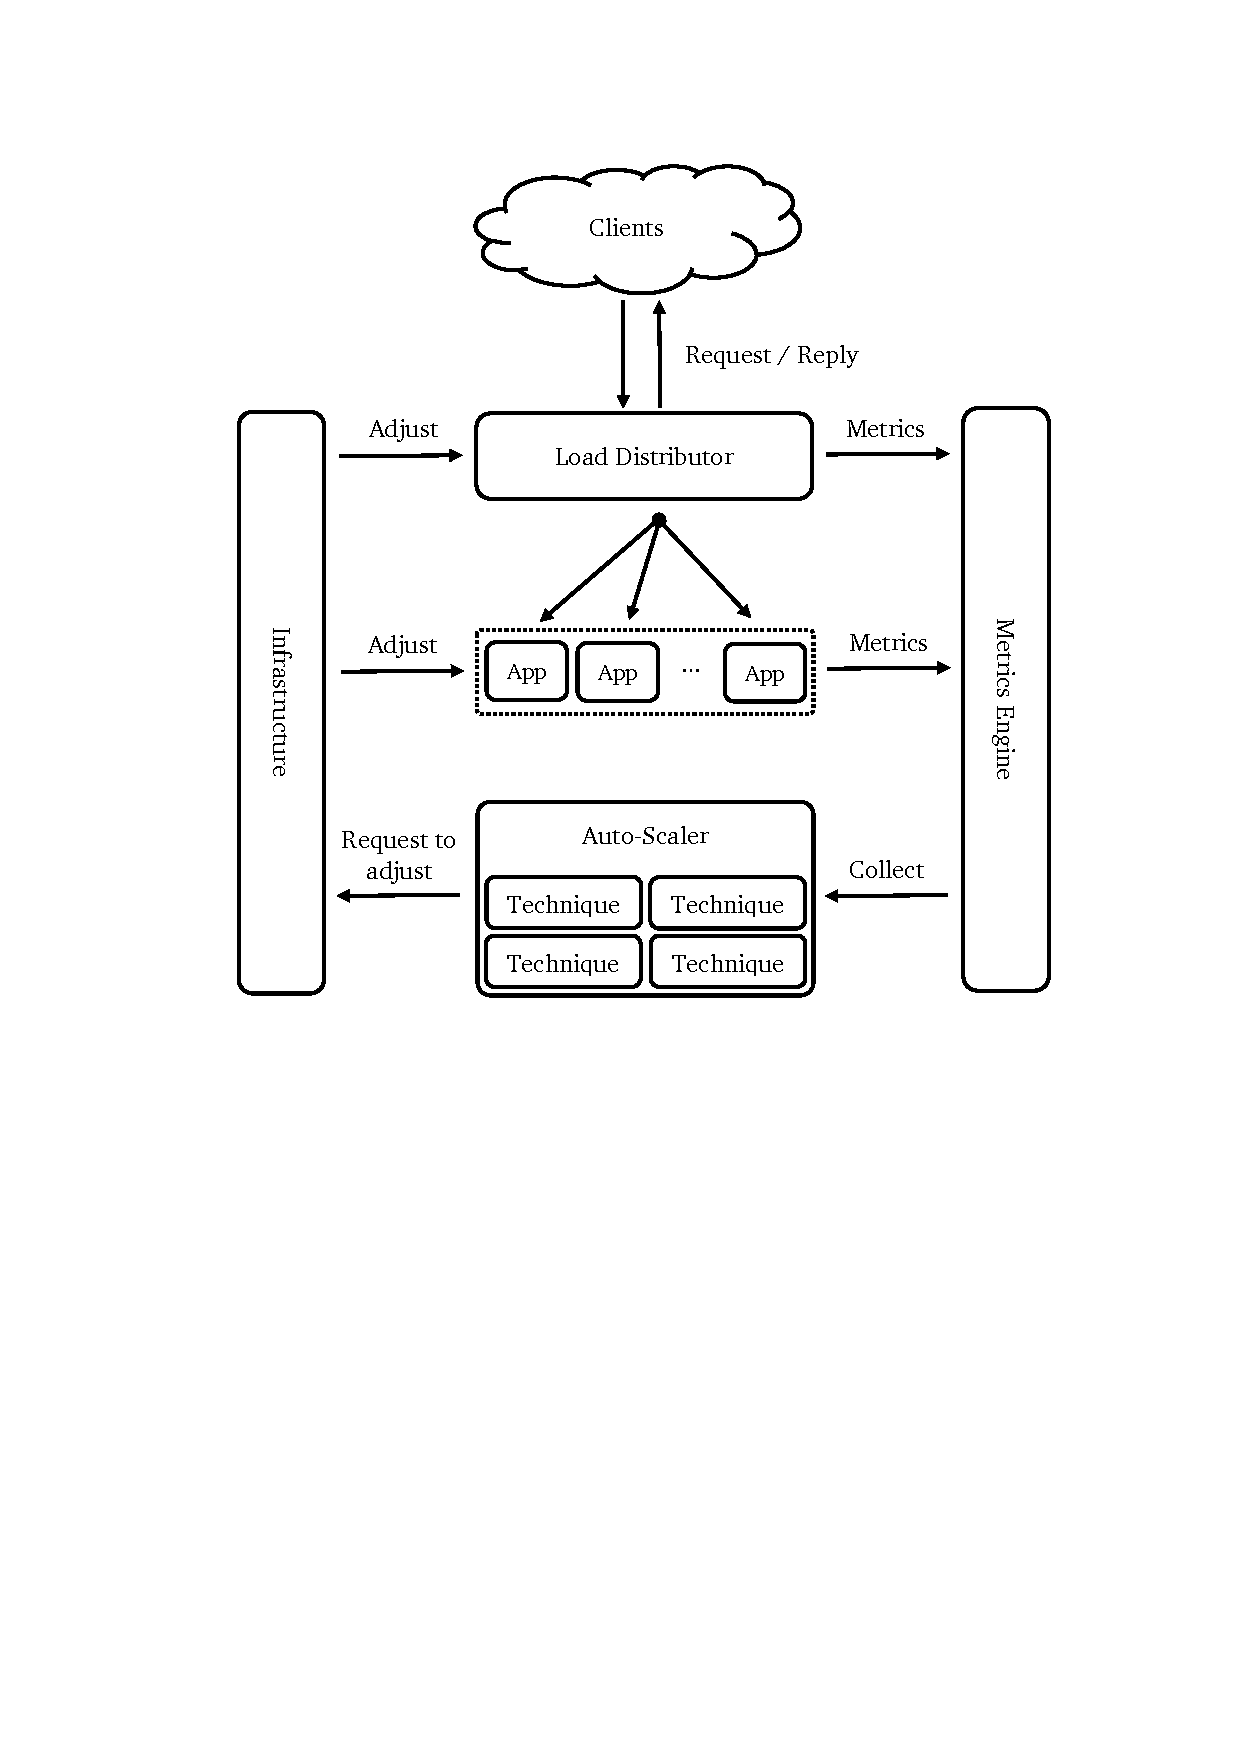
\includegraphics[clip, trim=3cm 13cm 2.5cm 2cm]{auto-scaler-arch.pdf}
    \caption{General Auto-Scaler Architecture}
    \label{fig:auto-scaler-arch}
\end{figure}

To make an effective decision, an Auto-Scaler need to consider application and its environment:
\begin{itemize}
    \item Cloud pricing model. In some 
    \item \emph{Service Level Objective} (SLO): Each application has its own set of predefined rules that shall not be violated during the process of acquiring and releasing resources. These rules typically context and application dependent. For example for web applications, one may define maximum round-trip latency that a user should wait until her request is fulfilled. 
    \item \emph{Unit of allocation}
\end{itemize}

In order to 
todo: write actions
todo: action horizental vs vertical

\section{Taxonomy of Auto-Scaling Techniques}
\label{ias:taxonomy}

\section{Conclusion}
\label{ias:conc}